\documentclass[aspectratio=43]{beamer}
\usepackage[latin1]{inputenc}
\usepackage{amsmath}
\usepackage{amsfonts}
\usepackage{amssymb}
\usepackage{makeidx}
\usepackage{graphicx}
\usepackage{array}

% Customization
\mode<presentation>{
\usetheme{CambridgeUS}
\usecolortheme{dolphin}
\setbeamertemplate{navigation symbols}{}
}

%\setbeamertemplate{footline}[frame number]

%TikZ diagrams
\usepackage{tikz}
\usetikzlibrary{patterns}
\usetikzlibrary{arrows,shapes}
\usetikzlibrary{shapes.multipart}
\usetikzlibrary{trees}
\usetikzlibrary{shapes.geometric}
\usetikzlibrary{matrix,arrows}
\usetikzlibrary{positioning}
\usetikzlibrary{calc,through}
\usetikzlibrary{decorations.pathreplacing}
\usepackage{pgffor}

% Define colors
\definecolor{darkgreen}{rgb}{0.0, 0.5, 0.13}
\definecolor{darkblue}{rgb}{0.0, 0.0, 0.55}
\definecolor{darkred}{rgb}{0.55, 0.0, 0.0}

% For using TikZ
\usetikzlibrary{decorations.pathmorphing}
\usetikzlibrary{decorations.markings}
\tikzset{
	vector/.style={decorate, decoration={snake,amplitude=3pt}, draw},
	gluon/.style={decorate, decoration={coil,amplitude=2.5pt},draw},
	provector/.style={decorate, decoration={snake,amplitude=2.5pt}, draw},
	antivector/.style={decorate, decoration={snake,amplitude=-2.5pt}, draw},
	fermion/.style={draw=black, postaction={decorate},
		decoration={markings,mark=at position .55 with {\arrow[draw=black,thick]{>}}}},
	fermionbar/.style={draw=black, postaction={decorate},
		decoration={markings,mark=at position .55 with {\arrow[draw=black,thick]{<}}}},
	fermionnoarrow/.style={draw=black},
	gluon/.style={decorate, draw=black,
		decoration={coil,amplitude=2.5pt, segment length=3pt}},
	gluon2/.style={decorate, draw=black,
		decoration={coil,amplitude=1.75pt, segment length=2.75pt}},
	scalar/.style={dashed,draw=black, postaction={decorate},
		decoration={markings,mark=at position .55 with {\arrow[draw=black]{>}}}},
	scalarbar/.style={dashed,draw=black, postaction={decorate},
		decoration={markings,mark=at position .55 with {\arrow[draw=black]{<}}}},
	scalarnoarrow/.style={dashed,draw=black},
	electron/.style={draw=black, postaction={decorate},
		decoration={markings,mark=at position .55 with {\arrow[draw=black]{>}}}},
	bigvector/.style={decorate, decoration={snake,amplitude=4pt}, draw},
}

% Blocks
\tikzstyle{block} = [draw, rectangle, minimum height = 3em, rounded corners, minimum width = 4em]
\tikzstyle{block2} = [draw, rectangle, minimum height = 3em, rounded corners, minimum width = 7em]
\tikzstyle{circle} = [draw, circle, radius = 1.5]
\tikzstyle{arrow} = [thick,->]
%************************************************************************************************************

% Title and author
\title[GP for theory uncertainties]{Machine Learning for the precision determination of Parton Distribution Functions}
\author{\textbf {Jes\'us Urtasun Elizari}}
%\institute{\textbf {University of Milan}}
\date{Milan, September 2020}

\begin{document}

% Front slide
\begin{frame}

	%\maketitle
	\vspace{1.0 cm}
	
	\center{\color{blue}Gaussian Process for the estimation of theory uncertainties}
	
	\vspace{0.25 cm}
	\center{Jes\'us Urtasun Elizari}
	\center{Italian Physical Society - Milan, September 2020}

	\begin{figure}
		\minipage{1\textwidth}
		
\includegraphics[width = 3.0 cm]{plots/unimi.png}
		\hfill
		
\includegraphics[width = 3.0 cm]{plots/n3pdf.png}
		\hfill
		
\includegraphics[width = 3.0 cm]{plots/erc.png}
		\endminipage
	\end{figure}

\end{frame}

% Introduction
\begin{frame}

	\frametitle{Outline}
	
	\begin{enumerate}
		\item {\color{blue}QCD in a nutshell}
		\begin{itemize}
			\item The Standard Model $\&$ strong interactions
			\item Parton Distribution Functions
			\item Factorization theorem
		\end{itemize}
		\item {\color{blue}Machine Learning}
		\begin{itemize}
			\item Motivation for Machine Learning
			\item Neural Networks $\&$ general strategy
		\end{itemize}
		\item {\color{blue}Gaussian Process and theory uncertainties}
		\begin{itemize}
			\item The NNPDF methodology
			\item Operator implementation in TensorFlow
			\item Results $\&$ Conclusions
		\end{itemize}
	\end{enumerate}
	
\end{frame}

% Quantum Chromodynamics in a nutshell
\begin{frame}
	
	\center{\color{blue} Quantum Chromodynamics in a nutshell}

\end{frame}

% The Standard model
\begin{frame}

	\frametitle{QCD in a nutshell}
	\framesubtitle{The Standard Model}

	\begin{figure}
		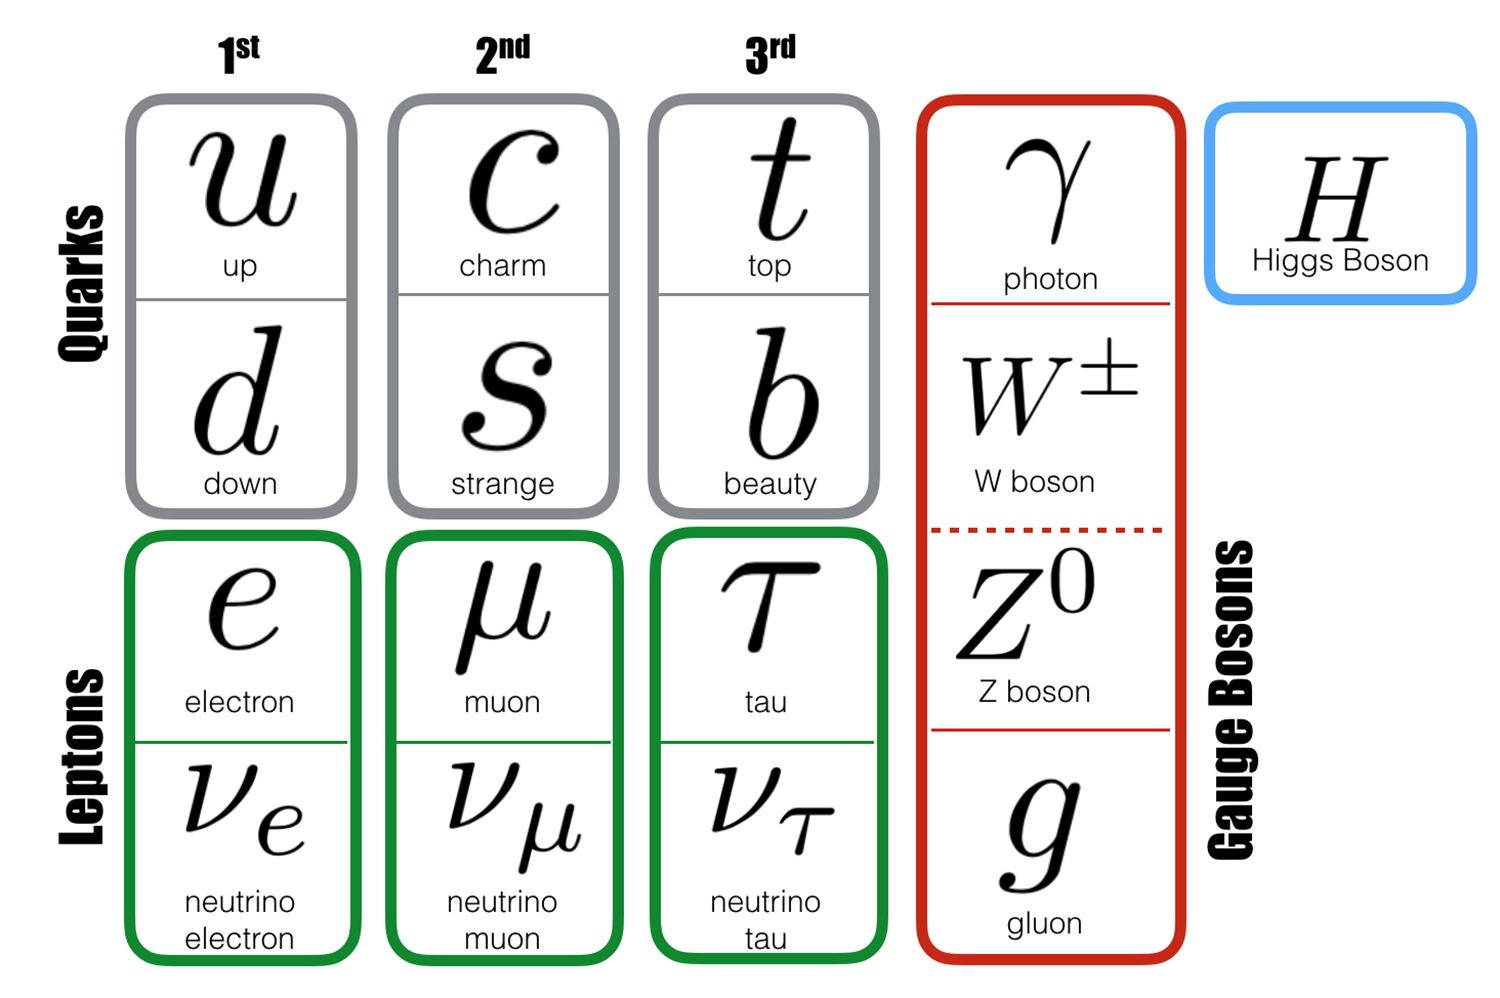
\includegraphics[width = 6 cm]{plots/SM.png}
	\end{figure}
 
	
	Quantum Field Theory describing physics at the TeV scale
	\begin{enumerate}
		\item Fermions composing matter
		\item Bosons mediating interactions
		\item Scalar Higgs generating mass
	\end{enumerate}	
	
\end{frame}

% Explore the proton structure
\begin{frame}

	\frametitle{QCD in a nutshell}
	\framesubtitle{Explore the strong interactions}
	
	How to explore proton's inner structure?
	
	\begin{figure}
		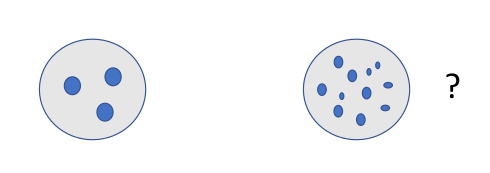
\includegraphics[width = 0.5\linewidth]{plots/protons.png}
	\end{figure}
	
	
	\begin{itemize}
		\item Point-like projectile on the object $\longrightarrow$ DIS
		\item Smash the two objects $\longrightarrow$ LHC physics
	\end{itemize}
	
	{\color{blue}"A way to analyze high energy collisions is to consider any hadron as a composition of point-like constituents $\longrightarrow$ \textbf{partons"} } R.Feynman, 1969 

\end{frame}

% Parton Distribution Functions
\begin{frame}

	\frametitle{QCD in a nutshell}
	\framesubtitle{Parton Distribution Functions}
	
	\begin{figure}
		\minipage{0.5\textwidth}
		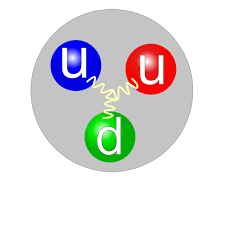
\includegraphics[width = 0.5\linewidth]{plots/proton.png}
		\endminipage\hfill
		\minipage{0.5\textwidth}
		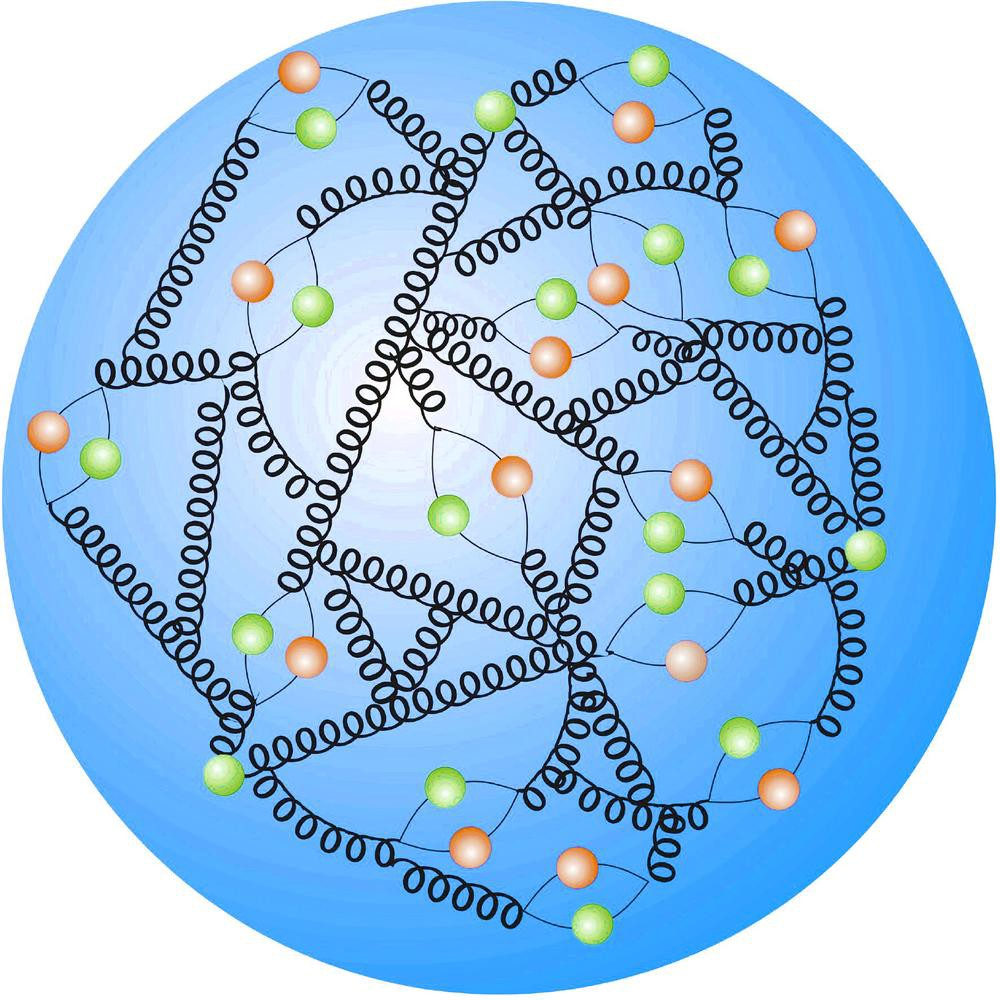
\includegraphics[width = 0.4\linewidth]{plots/proton2.jpg}
		\endminipage
	\end{figure}
	

	\begin{itemize}
		\item Hadrons made of partonic objects $\longrightarrow$ non perturbative physics
		\item Interactions take place only at partonic level
	\end{itemize}

	{\color{blue}Parton Distribution Functions: probability distribution of finding a particular parton (u, d, ..., g) carrying a fraction x of the proton's momentum}

\end{frame}

% Factorization theorem
\begin{frame}

	\frametitle{QCD in a nutshell}
	\framesubtitle{Factorization theorem}
	
	Observables in hadronic events $\longrightarrow$ $\sigma$ is hard to compute
	
	\begin{figure}
		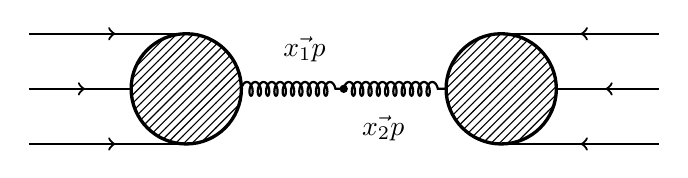
\begin{tikzpicture}
		% Incoming first proton 
		\draw [thick, fermion] (-4, 0.7)--(-2, 0.7);
		\draw [thick, fermion] (-4, 0)--(-2.7, 0);
		\draw [thick, fermion] (-4, -0.7)--(-2, -0.7);
		\draw [thick, very thick, pattern = north east lines] (-2, 0) circle [radius = 0.7];
		% Gluons
		\draw [thick, gluon] (-1.3, 0)--(0, 0);
		\draw [thick, gluon] (0, 0)--(1.3, 0);
		\node at (-0.5, 0.5) {$\vec{x_{1}p}$};
		\node at (0.5, -0.5) {$\vec{x_{2}p}$};
		\draw [thick, very thick, fill = black, pattern = north east lines] (0, 0) circle [radius = 0.03];
		% Incoming second proton
		\draw [thick, very thick, pattern = north east lines] (2, 0) circle [radius = 0.7];
		\draw [thick, fermionbar] (2, 0.7)--(4, 0.7);
		\draw [thick, fermionbar] (2.7, 0)--(4, 0);
		\draw [thick, fermionbar] (2, -0.7)--(4, -0.7);
		\end{tikzpicture}
	\end{figure}
	
	Factorize the problem $\longrightarrow$ Convolute the {\color{red}PDFs}  with the partonic ${\color{blue}\hat{\sigma}_{i j}}$
	
	\begin{equation}
		\sigma = \int_{0}^{1} dx_{1} \; dx_{2} \; {\color{red} f_{\alpha}(x_{1}, \mu_{F}) \ast f_{\beta}(x_{2}, \mu_{F})} \ast {\color{blue}\hat{\sigma}_{\alpha \beta}(\alpha_{s}(\mu_{R}), \mu_{F})} \; \nonumber
	\end{equation}
	
	\begin{itemize}
		\item Partonic {\color{blue}$\hat{\sigma}$} can be computed as perturbative series in $\alpha_{s}$
		\item {\color{red}PDFs} absorb the non perturbative effects, evaluated at $\mu_{F}$
	\end{itemize}

\end{frame}

% Parton Distribution functions (II)
\begin{frame}

	\frametitle{QCD in a nutshell}
	\framesubtitle{What PDFs look like}
	
	\begin{columns}
		\column{0.5\textwidth}
	
		\begin{itemize}
			\item Each parton has a different PDF \\ ${\color{blue}u(x)}, {\color{green}d(x)}, ..., {\color{red}g(x)}$
			\item PDFs are not predicted, and can not be measured
			\item PDFs are {\color{blue}extracted} from data
		\end{itemize}

		\column{0.5\textwidth}
		\begin{figure}
			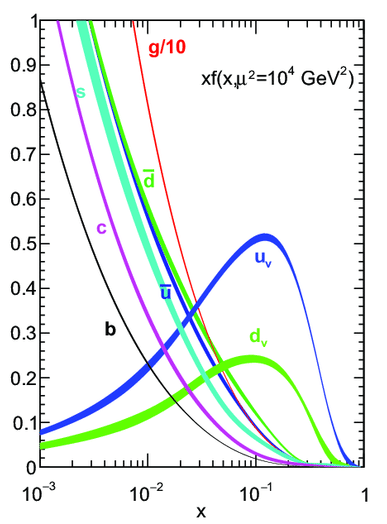
\includegraphics[width = 3.8 cm]{plots/PDF.png}
		\end{figure}

	\end{columns}

\end{frame}

% Machine Learning
\begin{frame}
	
	\center{\color{blue} Machine Learning}

\end{frame}

% Machine Learning introduction
\begin{frame}

	\frametitle{Machine learning}
	\framesubtitle{What is Machine Learning?}
	\begin{columns}
		
		\column{0.45\textwidth}
		
		\begin{enumerate}
			\item A subset of Artificial Intelligence (AI) algorithms 
			\item Used to solve \textit{complex} tasks like classification and regression
			\item Rely on comparison with data $\longrightarrow$ {\color{red}Learning}
		\end{enumerate}
		
		\column{0.45\textwidth}
		\begin{figure}[!htb]
			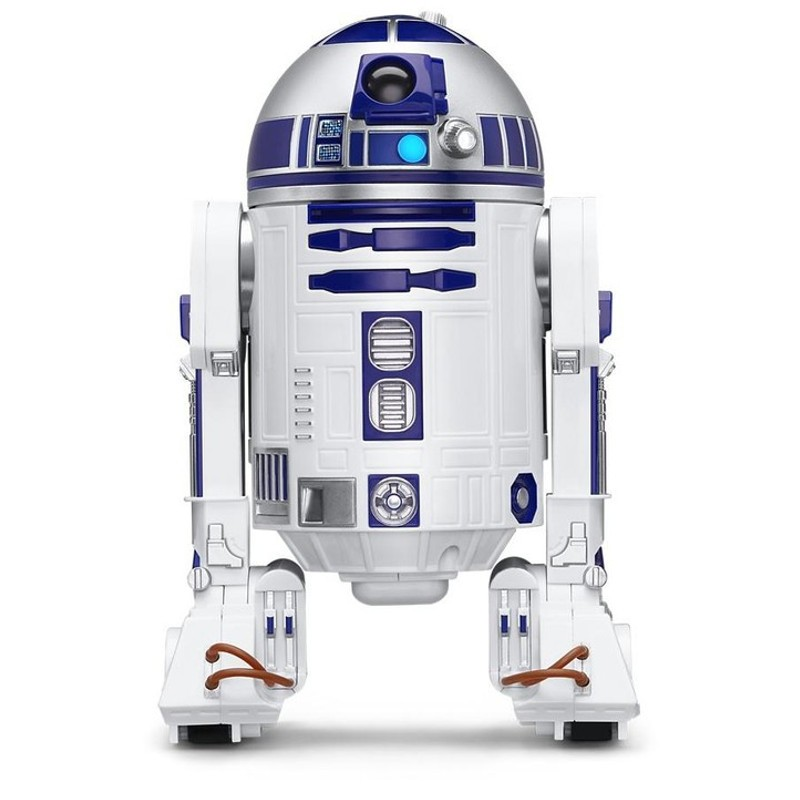
\includegraphics[width = \linewidth]{plots/r2d2.jpeg}
		\end{figure}
	
	\end{columns}

\end{frame}

% Building a ML model
\begin{frame}

	\frametitle{Machine learning}
	\framesubtitle{Building a ML model}
	
	\begin{figure}
		\minipage{0.33\textwidth}
		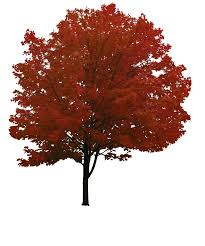
\includegraphics[width = \linewidth]{plots/tree2.jpeg}
		\endminipage\hfill
		\minipage{0.3\textwidth}
		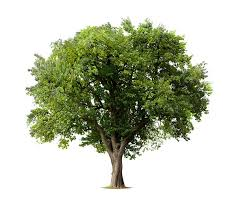
\includegraphics[width = \linewidth]{plots/tree1.jpeg}
		\endminipage\hfill
		\minipage{0.3\textwidth}
		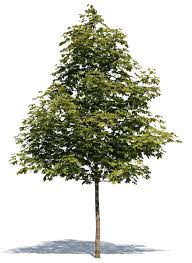
\includegraphics[width = \linewidth]{plots/tree3.jpeg}
		\endminipage
	\end{figure}

\end{frame}

% Building a ML model - strategy
\begin{frame}

	\frametitle{Machine learning}
	\framesubtitle{Building a Ml model}
	
		\begin{figure}
			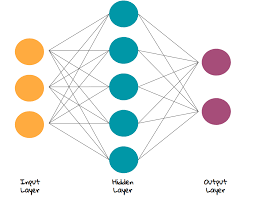
\includegraphics[width = 0.45\linewidth]{plots/NN.png}
		\end{figure}
		
	\begin{enumerate}
		\item Turn the input set into an array and build a {\color{red}random} prediction 
		\item Compare with truth and compute a {\color{blue}Loss} function
		\item Update the parameters in a specific way
	\end{enumerate}
	

\end{frame}

% Building a ML model - tree 1
\begin{frame}

	\frametitle{Machine learning}
	\framesubtitle{Building a ML model}
	
	\begin{figure}

		\minipage{0.33\textwidth}
		\begin{columns}
			\column{0.5\textwidth}
			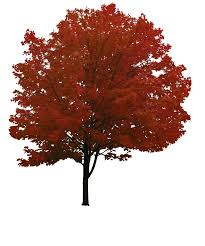
\includegraphics[width = \linewidth]{plots/tree2.jpeg}
			\column{0.5\textwidth}
			$\longrightarrow$
		\end{columns}
		\endminipage
		\hspace*{-1.25cm}	
		\minipage{0.3\textwidth}
		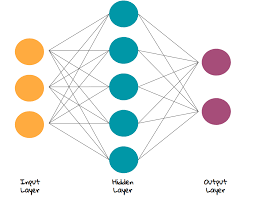
\includegraphics[width = 1.25\linewidth]{plots/NN.png}
		\endminipage
		\hspace*{0.75cm}
		\minipage{0.3\textwidth}
		$\longrightarrow$
		{\color{darkgreen}Tree \checkmark}
		\endminipage

	\end{figure}

\end{frame}

% Building a ML model - tree 2
\begin{frame}

	\frametitle{Machine learning}
	\framesubtitle{Building a ML model}
	
	\begin{figure}
		
		\minipage{0.33\textwidth}
		\begin{columns}
			\column{0.5\textwidth}
			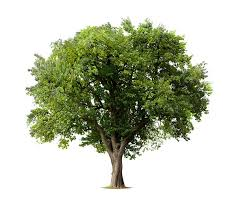
\includegraphics[width = \linewidth]{plots/tree1.jpeg}
			\column{0.5\textwidth}
			$\longrightarrow$
		\end{columns}
		\endminipage
		\hspace*{-1.25cm}	
		\minipage{0.3\textwidth}
		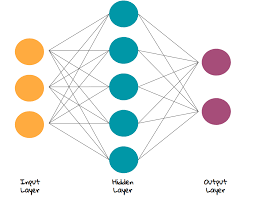
\includegraphics[width = 1.25\linewidth]{plots/NN.png}
		\endminipage
		\hspace*{0.75cm}
		\minipage{0.3\textwidth}
		$\longrightarrow$
		{\color{darkgreen}Tree \checkmark}
		\endminipage
		
	\end{figure}

\end{frame}

% Building a ML model - proton
\begin{frame}

	\frametitle{Machine learning}
	\framesubtitle{Building a ML model}
	
	\begin{figure}
		
		\minipage{0.33\textwidth}
		\begin{columns}
			\column{0.5\textwidth}
			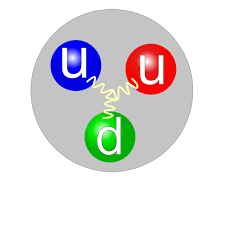
\includegraphics[width = \linewidth]{plots/proton.png}
			\column{0.5\textwidth}
			$\longrightarrow$
		\end{columns}
		\endminipage
		\hspace*{-1.25cm}	
		\minipage{0.3\textwidth}
		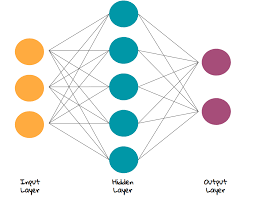
\includegraphics[width = 1.25\linewidth]{plots/NN.png}
		\endminipage
		\hspace*{0.75cm}
		\minipage{0.3\textwidth}
		$\longrightarrow$
		{\color{darkred}Not tree X}
		\endminipage
		
	\end{figure}

\end{frame}

% Building a ML model - tree 3
\begin{frame}
	
	\frametitle{Machine learning}
	\framesubtitle{Building a ML model}
	
	\begin{figure}
		
		\minipage{0.33\textwidth}
		\begin{columns}
			\column{0.5\textwidth}
			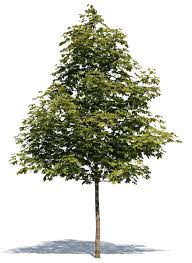
\includegraphics[width = \linewidth]{plots/tree3.jpeg}
			\column{0.5\textwidth}
			$\longrightarrow$
		\end{columns}
		\endminipage
		\hspace*{-1.25cm}	
		\minipage{0.3\textwidth}
		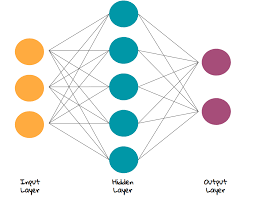
\includegraphics[width = 1.25\linewidth]{plots/NN.png}
		\endminipage
		\hspace*{0.75cm}
		\minipage{0.3\textwidth}
		$\longrightarrow$
		{\color{darkgreen}Tree \checkmark}
		\endminipage
		
	\end{figure}

\end{frame}

% Loss function
\begin{frame}

	\frametitle{Machine Learning}
	\framesubtitle{Loss function}
	
	\begin{columns}
		
		\column{0.45\textwidth}
		\begin{figure}
			\centering
			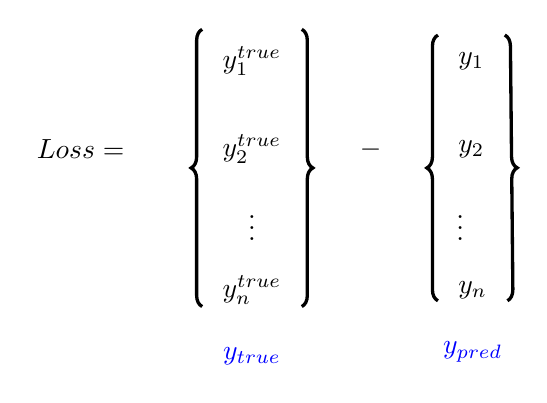
\begin{tikzpicture}
			
				% List of ypred
				\node (y1) {$y_{1}^{true}$};
				\node[below = 0.5 cm of y1] (y2) {$y_{2}^{true}$};
				\node[below = 0.2 cm of y2] (yd) {\vdots};
				\node[below = 0.2 cm of yd] (yn) {$y_{n}^{true}$};
				\node[below = 0.3 cm of yn] (ygrid) {\color{blue}$y_{true}$};
				\coordinate[right = 0.3 cm of y2] (ry2);
				
				% Braces
				\draw[decorate, decoration={brace, amplitude = 4pt, raise = 1pt}, very thick]
				($(y1.north east) + (0.1, 0.1)$) -- ($(yn.south east) + (0.1, 0.1)$);
				\draw[decorate, decoration={brace, amplitude = 4pt, raise = 1pt}, very thick]
				($(yn.south west) + (-0.1, 0.1)$) -- ($(y1.north west) + (-0.1, 0.1)$);
				
				% Loss function
				\node[right = 0.75 cm of y2] (loss) {$-$};
				
				% List of ytrue
				\node[right = 2.0 cm of y1] (y1t) {$y_{1}$};
				\node[right = 2.0 cm of y2] (y2t) {$y_{2}$};
				\node[right = 2.3 cm of yd] (ydt) {\vdots};
				\node[right = 2.0 cm of yn] (ynt) {$y_{n}$};
				\node[below = 0.3 cm of ynt] (ygrid) {\color{blue}$y_{pred}$};
				\coordinate[left = 0.3 cm of y2] (ly2t);
				\coordinate[right = 0.3 cm of y2] (ry2t);
			
				% Braces
				\draw[decorate, decoration = {brace, amplitude = 4pt, raise = 1pt}, very thick]
				($(y1t.north east) + (0.1, 0.1)$) -- ($(ynt.south east) + (0.1, 0.1)$);
				\draw[decorate, decoration = {brace, amplitude = 4pt, raise = 1pt}, very thick]
				($(ynt.south west) + (-0.1, 0.1)$) -- ($(y1t.north west) + (-0.1, 0.1)$);
			
				% Loss function
				\node[left = 1.0 cm of y2] (loss) {$Loss = $};
							
			\end{tikzpicture}
		\end{figure}

		\column{0.35\textwidth}
		\begin{enumerate}
			\item Compute a loss function
			\begin{equation*}
				L = \sum\limits_{i = 1}^{N} \big( y_{i}^{true} - y_{i}^{pred} \big)^{2}
			\end{equation*}
			\item Perfect prediction will mean $L = 0$
		\end{enumerate}

	\end{columns}

\end{frame}

% Loss function - gradient
\begin{frame}

	\frametitle{Machine Learning}
	\framesubtitle{Loss function}

	\begin{columns}
		
		\column{0.45\textwidth}
		
		\begin{enumerate}
			\item Loss is a function of weights and bias $L = L(w, b)$
			\item Compute gradient $\nabla_{w_{ij}} L$ to look for the minimum of L
		\end{enumerate}
		
		\column{0.45\textwidth}
	
			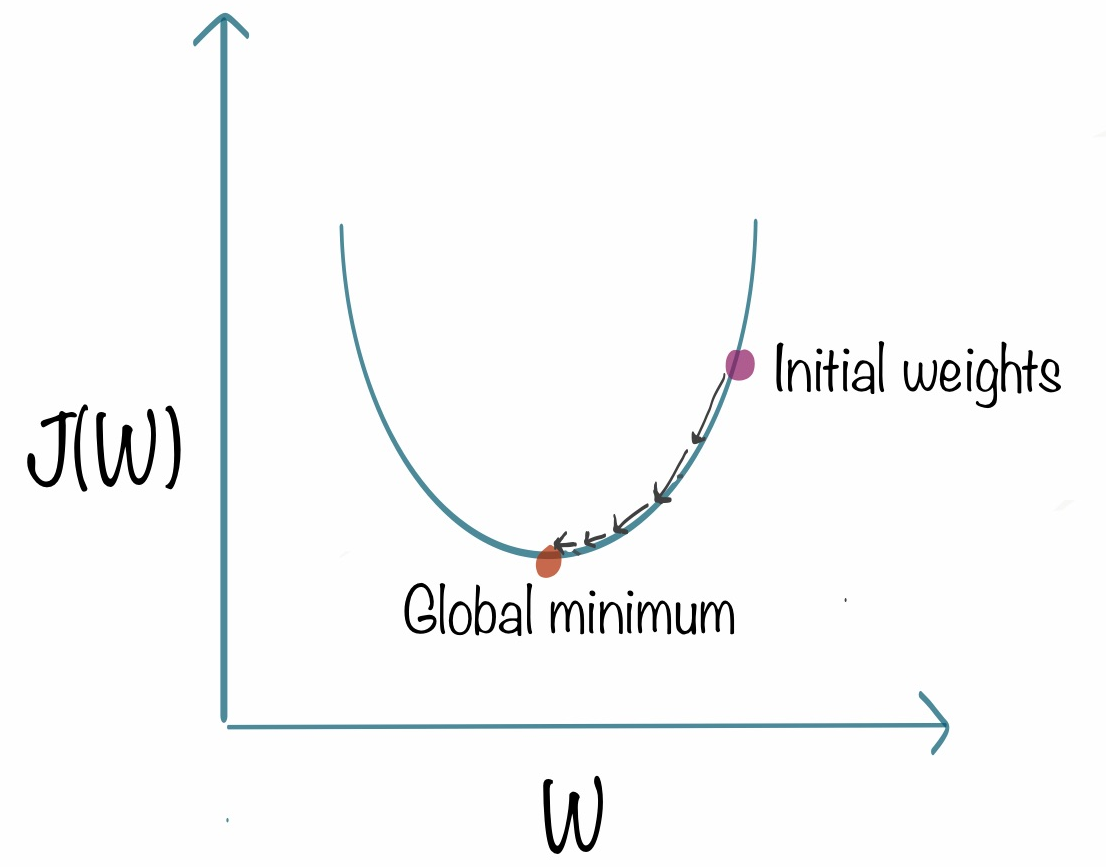
\includegraphics[width = \linewidth]{plots/loss.png}
			
	\end{columns}

\end{frame}

% Update rule
\begin{frame}

	\frametitle{Machine Learning}
	\framesubtitle{Update rule}
	
	\begin{columns}
		
		\column{0.45\textwidth}
		
		Update the parameters of the network following the gradient descend
		
		\begin{align}
			w_{ij} \longrightarrow w_{ij} - \alpha \nabla L \nonumber \\
			b_{i} \longrightarrow b_{i} - \alpha \nabla L  \nonumber
		\end{align}
		
		Where $\alpha$ is the learning rate
		
		\column{0.4\textwidth}
		
		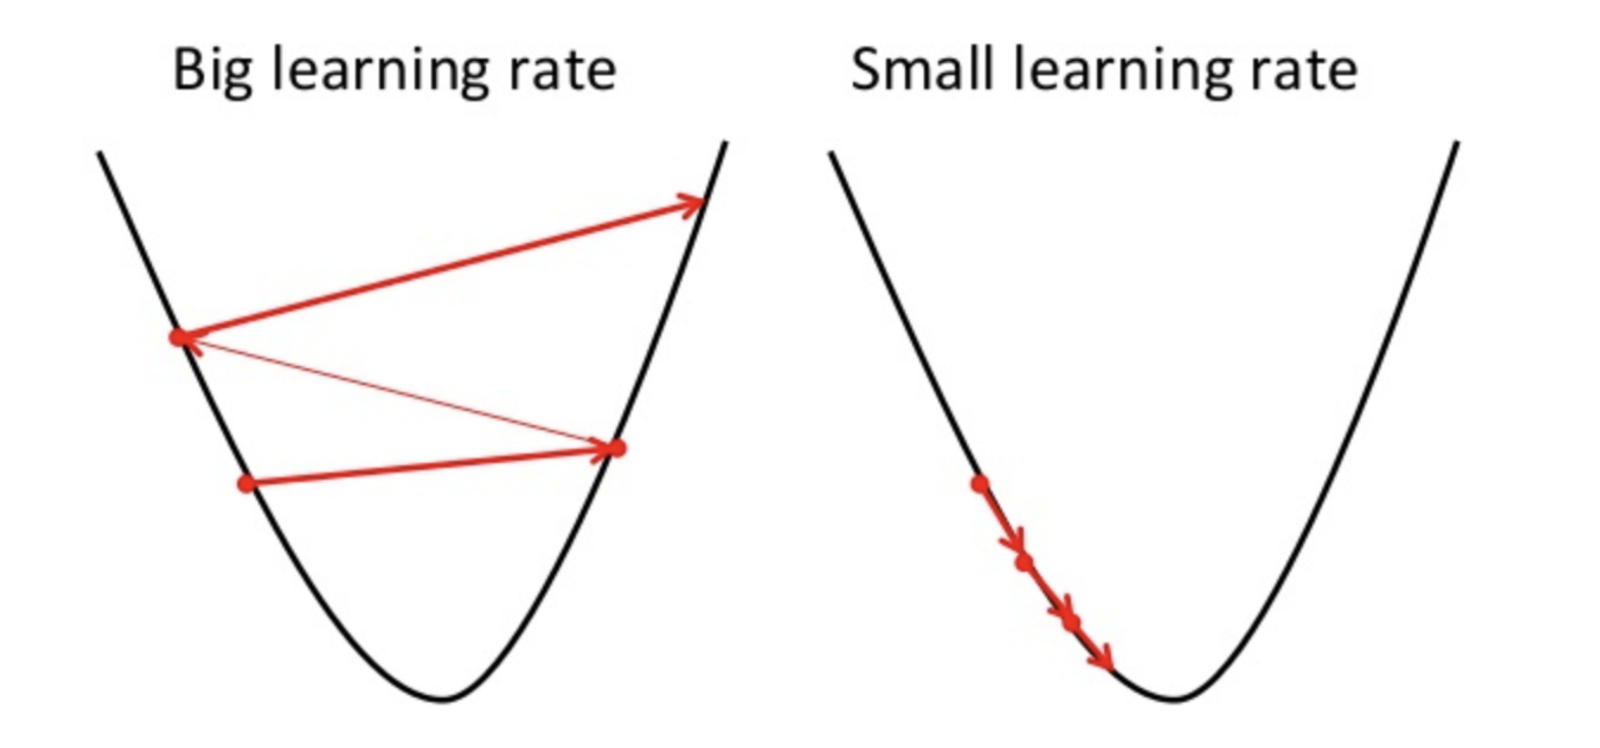
\includegraphics[width = 1.25 \linewidth]{plots/loss2.png}
		
	\end{columns}

\end{frame}

% The N3PDF project
\begin{frame}

	\center{\color{blue} The N3PDF project}
	\center{\color{blue} Machine Learning for the precision determination of PDFs}

\end{frame}

% NNPDF methodology
\begin{frame}

	\frametitle{The N3PDF project}
	\framesubtitle{The NNPDF methodology}
	
	Factorize the problem $\longrightarrow$ Convolute the {\color{red}PDFs}  with the partonic ${\color{blue}\hat{\sigma}_{i j}}$
	
	\begin{equation}
	\sigma = \int_{0}^{1} dx_{1} \; dx_{2} \; {\color{red} f_{\alpha}(x_{1}, \mu_{F}) \ast f_{\beta}(x_{2}, \mu_{F})} \ast {\color{blue}\hat{\sigma}_{\alpha \beta}(\alpha_{s}(\mu_{R}), \mu_{F})} \; \nonumber
	\end{equation}
	
	\begin{itemize}
		\item Partonic ${\color{blue}\hat{\sigma}_{\alpha\beta}}$ is computed perturbatively. Hadronic $\sigma$ is measured.
		\item Use a Neural Networks to generate (\textit{fit}) the PDFs
		\item Generate a vector of observables $\sigma_{N}$ to be compared with data
	\end{itemize}
	
	\begin{equation}
	\sigma_{N} = \sum_{i, j, \alpha, \beta} {\color{red}f_{\alpha}(x_{i}) \; f_{\beta}(x_{j})} \; {\color{blue}\hat{\sigma}_{N i j \alpha \beta}} \; \nonumber
	\end{equation}

\end{frame}

% General structure of a fit
\begin{frame}

	\frametitle{The N3PDF project}
	\framesubtitle{General structure of n3fit}

	\begin{figure}[!htb]
		\minipage{0.32\textwidth}
		
\includegraphics[width = 0.5\linewidth]{plots/TF.png}
		\endminipage\hfill
		\minipage{0.5\textwidth}
		
\includegraphics[width = 0.5\linewidth]{plots/Keras.png}
		\endminipage\hfill
	\end{figure}

	\begin{itemize}
		\item Use TensorFlow and Keras to determine the PDFs
		\item See paper by S.Carraza - J.Cruz-Martinez \\
		{\color{blue}"Towards a new generation of parton densities\\ with deep learning models",\\ https://arxiv.org/abs/1907.05075}
	\end{itemize}

\end{frame}

% General structure
\begin{frame}

	\frametitle{The N3PDF project}
	\framesubtitle{General structure of n3fit}

	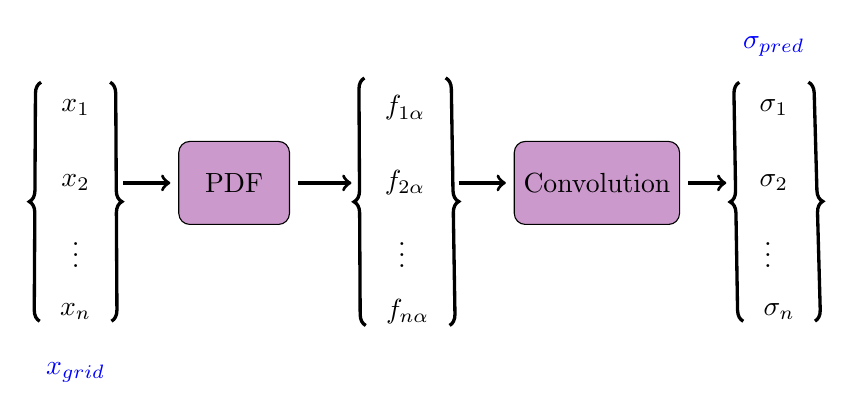
\begin{tikzpicture}
	
		% List of xs
		\node (x1) {$x_{1}$};
		\node[below = 0.5 cm of x1] (x2) {$x_{2}$};
		\node[below = 0.2 cm of x2] (xd) {\vdots};
		\node[below = 0.2 cm of xd] (xn) {$x_{n}$};
		\node[below = 0.3 cm of xn] (xgrid) {\color{blue}$x_{grid}$};
		\coordinate[right = 0.3 cm of x2] (rx2);
		% Braces
		\draw[decorate, decoration={brace, amplitude = 4pt, raise = 1pt}, very thick]
		($(x1.north east) + (0.1, 0.1)$) -- ($(xn.south east) + (0.1, 0.1)$);
		\draw[decorate, decoration={brace, amplitude = 4pt, raise = 1pt}, very thick]
		($(xn.south west) + (-0.1, 0.1)$) -- ($(x1.north west) + (-0.1, 0.1)$);
		
		% PDF layer
		\node[block, fill = violet!40, right = 1.0 cm of x2] (pdf) {PDF};
		\coordinate[left = 0.1 cm of pdf] (lpdf);
		\coordinate[right = 0.1 cm of pdf] (rpdf);
		
		% List of pdfs
		\node[right = 3.5 cm of x1] (f1) {$f_{1 \alpha}$};
		\node[right = 3.5 cm of x2] (f2) {$f_{2 \alpha}$};
		\node[right = 3.8 cm of xd] (fd) {\vdots};
		\node[right = 3.5 cm of xn] (fn) {$f_{n \alpha}$};
		\coordinate[left = 0.3 cm of f2] (lf2);
		\coordinate[right = 0.3 cm of f2] (rf2);
		% Braces
		\draw[decorate, decoration = {brace, amplitude = 4pt, raise = 1pt}, very thick]
		($(f1.north east) + (0.1, 0.1)$) -- ($(fn.south east) + (0.1, 0.1)$);
		\draw[decorate, decoration = {brace, amplitude = 4pt, raise = 1pt}, very thick]
		($(fn.south west) + (-0.1, 0.1)$) -- ($(f1.north west) + (-0.1, 0.1)$);
		
		% Convolution layer
		\node[block, fill = violet!40, right = 1.0 cm of f2] (conv) {Convolution};
		\coordinate[left = 0.1 cm of conv] (lconv);
		\coordinate[right = 0.1 cm of conv] (rconv);
		\coordinate[below = 0.1 cm of conv] (bconv);
		
		% List of y
		\node[right = 4.0 cm of f1] (y1) {$\sigma_{1}$};
		\node[right = 4.0 cm of f2] (y2) {$\sigma_{2}$};
		\node[right = 4.3 cm of fd] (yd) {\vdots};
		\node[right = 4.0 cm of fn] (yn) {$\sigma_{n}$};
		\node[above = 0.3 cm of y1] (ypred) {\color{blue}$\sigma_{pred}$};
		\coordinate[left = 0.3 cm of y2] (ly2);
		% Braces
		\draw[decorate, decoration = {brace, amplitude = 4pt, raise = 1pt}, very thick]
		($(y1.north east) + (0.1, 0.1)$) -- ($(yn.south east) + (0.1, 0.1)$);
		\draw[decorate, decoration = {brace, amplitude = 4pt, raise = 1pt}, very thick]
		($(yn.south west) + (-0.1, 0.1)$) -- ($(y1.north west) + (-0.1, 0.1)$);
		
		% Connect all nodes defined above
		\draw[arrow, very thick] (rx2) -- (lpdf);
		\draw[arrow, very thick] (rpdf) -- (lf2);
		\draw[arrow, very thick] (rf2) -- (lconv);
		\draw[arrow, very thick] (rconv) -- (ly2);
	
	\end{tikzpicture}
	
	\begin{enumerate}
		\item Build a NN to compute $\sigma_{pred}$ observables from a grid $x_{i}$
		\item Compute $\chi^{2}$ loss function by comparing with data
		\item Update values of PDF $\longrightarrow$ {\color{violet} Fit}
	\end{enumerate}

\end{frame}

% Conclusions
\begin{frame}
	
	\frametitle{Summary $\&$ Conclusions}

	\begin{enumerate}
		\item PDFs are required to have accurate predictions in high energy physics
		\item ML provides a new way of determine the PDFs
		\item Operator implementation leads to memory saving by taking full control on the computation
	\end{enumerate}

\end{frame}

% Thank you
\begin{frame}

	\center {\color{blue} Thank you!}
	
	\begin{figure}
		
\includegraphics[width = 3 cm]{plots/thinking2.png}
	\end{figure}
	
	{\small \color{blue} This project has received funding from the European Union$'$s Horizon 2020 research and innovation program under grant agreement No 740006.}

\end{frame}

\end{document}